\textbf{Acknowledgement: }\textit{I would like to thank Dr Saulo de Oliveira for his contributions to this chapter. He kindly provided his time and expertise to generating SAINT2 structure predictions included in the analysis presented in this chapter.}

\section{Introduction}
To-date, the recommended \textit{ab initio} protein structure prediction protocol for optimal AMPLE performance is ROSETTA \cite{Keegan2015-zb, Thomas2017-sh, Thomas2015-wu, Bibby2012-lm}. This recommendation is based primarily on the superiority of the decoy quality compared to other modelling algorithms, which was recently reaffirmed by the lastest CASP12 experiments \cite{Abriata2018-lu,Ovchinnikov2017-wp}. However, \textcite{Keegan2015-zb} demonstrated that the alternative \textit{ab initio} structure prediction protocol QUARK provides a suitable alternative to ROSETTA in AMPLE. Although inferior in the total number of structure solutions, QUARK decoys are a suitable ROSETTA alternative in most cases \cite{Keegan2015-zb}. In particular, given ROSETTA's challenging installation procedure, availability limited to POSIX operating systems, requirement for large disk space and computationally expensive algorithm, QUARK's online server has been a very attractive alternative for AMPLE users.

Whilst ROSETTA and QUARK are amongst the best \textit{ab initio} structure prediction algorithms currently available \cite{Abriata2018-lu}, other algorithms have been developed over the last two decades \cite[e.g.,][]{Jones2001-mc,Ellis2010-zs,Adhikari2015-lb,Xu2012-jf,Marks2011-os,Wang2016-ar}. Although most of these algorithms utilise fragment-assembly algorithms similar to ROSETTA and QUARK, their procedures for fragment selection or assembly is substantially different \cite{Ellis2010-zs,Jones2001-mc}. Furthermore, predicted contact information has recently seen a spike in accuracy. This invaluable source of information is introduced differently in each protocol, and thus might have profound effects on the resulting decoy quality. In particular, physics-based algorithms relying largely on this information are an interesting alternative to fragment-based approaches \cite{Adhikari2015-lb,Marks2011-os,Wang2016-ar}.

CONFOLD2 \cite{Adhikari2018-lj}, a distance-geometry based algorithm, uses predicted secondary structure and contact information to rapidly generate \textit{ab initio} decoys. Unlike other algorithms, CONFOLD2's algorithm is driven almost entirely by the contact information to explore the fold space. Different contact selection thresholds are used to not limit the search space to a fixed, predefined selection. CONFOLD2 generates slightly less accurate decoys compared to ROSETTA, however outperforms it in speed and simplicity of installation \cite{Adhikari2018-lj,Michel2017-xh}.

FRAGFOLD \cite{Jones2001-mc}, a fragment-assembly based algorithm, generates decoys in a similar fashion to ROSETTA and QUARK. However, FRAGFOLD does not rely on large structural libraries for fragment extraction. Instead, it provides a relatively small library of supersecondary structural fragments and short length fragments, which were extracted from high resolution protein structures. Since the generalised fragment library is shipped with FRAGFOLD, and target-specific fragments are extracted based on secondary structure and a sequence-based threading score, fragment library generation is fast and easy compared to ROSETTA \cite{Kosciolek2014-bt}.

SAINT2 \cite{De_Oliveira2017-sg}, a further fragment-assembly based algorithm is substantially different to most others. SAINT2 attempts \textit{ab initio} structure prediction sequentially, starting from either terminus of the target sequence \cite{De_Oliveira2017-sg}. Furthermore, SAINT2 uses FLIB \cite{De_Oliveira2015-kb} for fragment picking, an algorithm shown to outperform ROSETTA's equivalent NNMake \cite{Gront2011-sv} in precision with very similar coverage.

Since some of these algorithms are readily available and often easier to install without the overhead of large databases for fragment picking, the work in this study focused on exploring three alternative \textit{ab initio} structure prediction algorithms and their value in unconventional \gls{mr}. The \textit{ab initio} structure prediction protocols CONFOLD2 \cite{Adhikari2018-lj}, FRAGFOLD \cite{Jones2001-mc} and SAINT2 \cite{De_Oliveira2017-sg}, were explored given their substantially different approaches to AMPLE's current default ROSETTA \cite{Rohl2004-dj}.

\section{Materials \& Methods}
\subsection{Target selection}
This study was conducted using all 27 targets from the PREDICTORS dataset (\cref{sec:methods_dataset_predictors}).

\subsection{Contact prediction}
Residue-residue contact information was predicted for 18 out of 27 targets using METAPSICOV v1.04 \cite{Jones2015-vq}.

Secondary structure and solvent exposure were predicted using PSIPRED v4.0 \cite{Jones1999-ed} and SOLVPRED (shipped with METAPSICOV v1.04), respectively. The \gls{msa} for coevolution-based contact prediction was generated using HHBLITS \cite{Remmert2011-kt} against the \texttt{uniprot20\_2016\_02} database. CCMPRED v0.3.2 \cite{Seemayer2014-zp}, FREECONTACT v1.0.21 \cite{Kajan2014-bx} and PSICOV v2.1b3 \cite{Jones2012-ks} were used by METAPSICOV to generate contact predictions.

METAPSICOV STAGE 1 contact predictions were used in \textit{ab initio} structure prediction since they result in more accurate structure predictions than METAPSICOV STAGE 2 results \cite{Jones2015-vq}.

\subsection{\textit{Ab initio} structure prediction} \label{sec:ample_saint2_modelling}
The ROSETTA 3- and 9-residue fragment libraries for each target were generated using the ROBETTA online server (\url{http://robetta.bakerlab.org/}). The option to ``Exclude Homologues'' was selected to avoid inclusion of homologous fragments. Each target sequence and its fragments were subjected to ROSETTA v2015.22.57859 \cite{Rohl2004-dj} and 1,000 decoys per target generated with AMPLE v1.2.0 ROSETTA default options. Top-$L$ (where $L$ corresponds to the number of residues in the target chain) contact pairs were used in combination with the \textit{FADE} ROSETTA energy function. For further details see \cref{chap:proof_of_principle} or \textcite{Michel2014-eg}.

The CONFOLD2 decoys were generated using CONFOLD2 v2.0 \cite{Adhikari2018-lj}, which uses \gls{cns} v1.3 \cite{Brunger1998-sz} to drive the modelling. Default parameters were used except for the number of decoys per run, which was increased from 20 to 25 with \texttt{-mcount 25}. CONFOLD2 varies the number of contacts included in each separate modelling run, ranging from $L/10$ to $4L$ with increments of $L/10$. Thus, the CONFOLD2 protocol yields a total of 40 separate modelling runs generating 25 decoys each.

The FRAGFOLD decoys were generated using FRAGFOLD v4.80 \cite{Jones2001-mc} with default options. Homologous fragments were removed from the shipped library  by excluding all entries with \gls{pdb} identifiers identical to those retrieved from the ROBETTA server. All contact pairs were used according to FRAGFOLD's internal protocol.

The fragment libraries for SAINT2 were generated using FLIB \cite{De_Oliveira2015-kb}, which generates on average ~30 fragments per target position that are 6 to 20 residues long. Homologous fragments were removed from the final fragment list using the \gls{pdb} identifiers obtained from the ROBETTA online server. The secondary structure prediction and solvent accessibility scores were identical to those obtained from the ROBETTA server. SAINT2 was used for decoy generation, and 1,000 decoys generated per target. The procedure and parameters were identical to those described in Supplementary Information (p. 16) by \textcite{De_Oliveira2017-sg}.

\subsection{Molecular Replacement}
All decoy sets were subjected to AMPLE v1.2.0 and CCP4 v7.0.28. Default options were chosen with the following exceptions: decoys in all 10 clusters were used, subcluster radii thresholds were set to 1 and 3\AA, and side-chain treatments were set to \texttt{polyala} only. This change in protocol from AMPLE's initial mode of operation \cite{Bibby2012-lm} was shown to be advantageous in most cases by \textcite{Thomas2017-qu}, and thus trialled in this context.  Each \gls{mr} run was assessed using the SHELXE criteria, where a minimum \gls{cc} of 25.0 and \gls{acl} of 10 was required (\cref{sec:methods_mr_success}). R-values of $<0.45$ after model building were not part of the success criteria in this study.

\section{Results}
The purpose of this study was to investigate the usefulness of alternative \textit{ab initio} structure prediction algorithms in AMPLE. Three promising leads widely used in the \textit{ab initio} modelling experiments were examined and compared against AMPLE's current algorithm of choice. This led to a direct comparison of the algorithms ROSETTA \cite{Rohl2004-dj}, CONFOLD2 \cite{Adhikari2018-lj}, FRAGFOLD \cite{Jones2001-mc} and SAINT2 \cite{De_Oliveira2017-sg}. All four algorithms have recently seen great improvements through the use of residue-residue contact information, which was predicted for two-thirds of the targets using the METAPSICOV \cite{Jones2015-vq} algorithm.

\subsection{Alignment depth and contact prediction precision}
The first step in this study was the prediction of residue-residue contacts using the metapredictor METAPSICOV for 18 targets in the PREDICTORS dataset \cite{Jones2015-vq}. Since we attempted to test each of the structure prediction boundaries in extreme cases, a variety of targets with different alignment depths were chosen. The alignment depth --- i.e., the number of effective sequences --- of METAPSICOV-generated HHBLITS alignments ranges from 431 to 6,186 across all targets (\cref{fig:ample_saint2_alndepth}). Six targets contain at least 200 and less than 1000 sufficiently-diverse sequences, whilst the remaining 16 targets contain more than 1,000 effective sequences.

\begin{figure}[H]
    \centering
    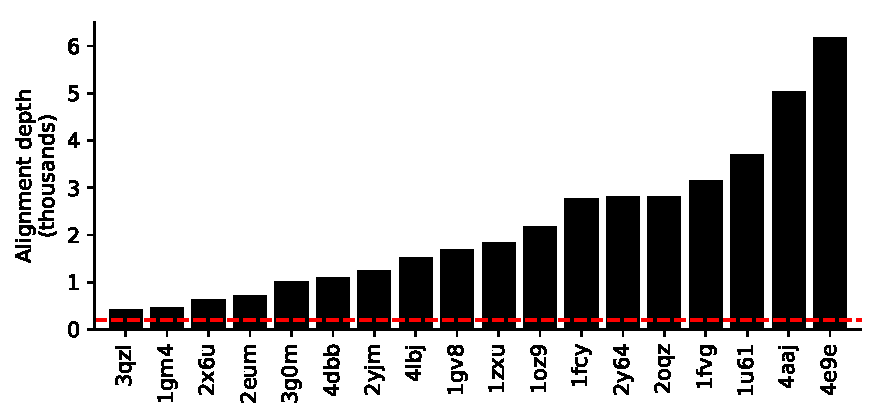
\includegraphics[width=\textwidth]{ample_saint2_alndepth.pdf}
    \caption[Distribution of alignment depth for subset of targets in the PREDICTORS dataset.]{Distribution of HHBLITS alignment depth for subset of targets in the PREDICTORS dataset. Red line indicates alignment depth threshold of 200 sequences \cite{Simkovic2017-xs}.}
    \label{fig:ample_saint2_alndepth}
\end{figure}

Coevolution-based contact predictors rely heavily on the alignment depth for accurate contact predictions. In this work, these findings are further confirmed. Sequence alignments with depths of less than 1,000 sequences produce contact predictions with lower precision scores across a number of cutoffs compared to those with deeper alignments (\cref{fig:ample_saint2_conprec}). Given the alignment depths and top-$L$ contact predictions, a positive correlation between the two is found (Spearman's $\rho=0.57$, p-value $<0.02$). A moving average analysis shows that those contact predictions based on alignments with more than 1,000 effective sequences yield better precision scores of at least 0.09 units up to 0.34 units. The difference between the two moving average curves highlights that the difference is greater at lower cutoff values, i.e. only the very best contacts are included in the selection. This difference declines more drastically for targets with deeper alignments (\cref{fig:ample_saint2_conprec}).

\begin{figure}[H]
    \centering
    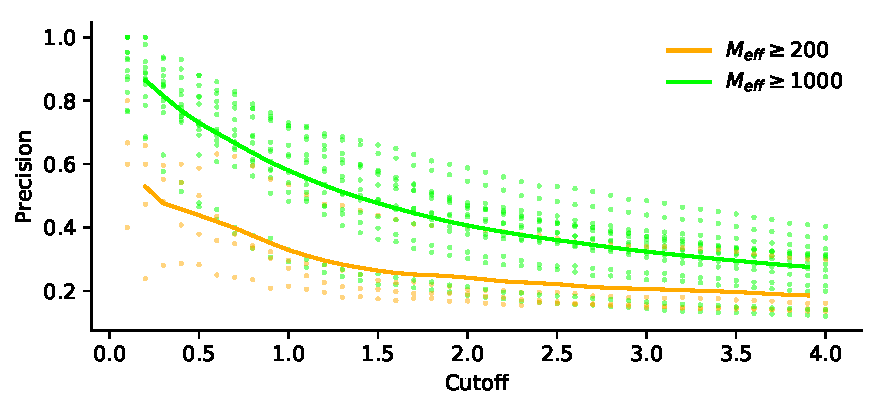
\includegraphics[width=\textwidth]{ample_saint2_conprec.pdf}
    \caption[Contact predicion analysis for numerous contact selection cutoffs]{Contact precision analysis for numerous contact selection cutoffs for targets with alignment depths of more than 200 and more than 1,000 sequences. Lines indicate moving averages for both categories with a window size of three residues. $M_{eff}$ refers to the alignment depth (number of effective sequences).}
    \label{fig:ample_saint2_conprec}
\end{figure}

\subsection{Comparison of decoy quality}
One main interest of the work presented in this chapter is the comparison of the quality of decoys predicted with four \textit{ab initio} structure prediction algorithms. To-date, no such direct comparison exists on the same dataset, and thus might provide direct insights into the performance of each.

\begin{figure}[H]
    \centering
    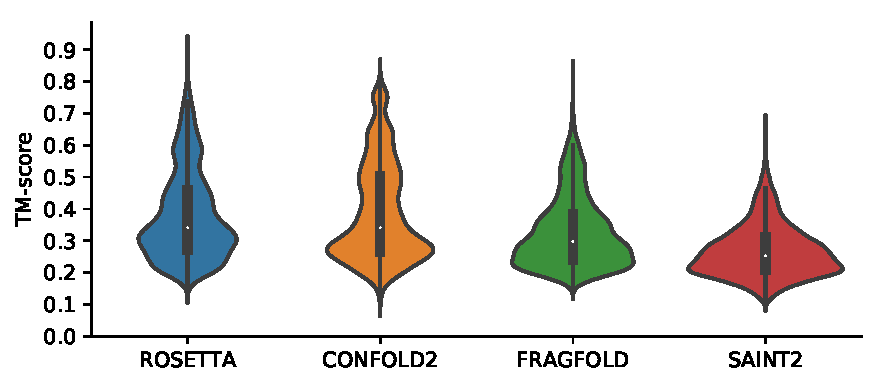
\includegraphics[width=\textwidth]{ample_saint2_tmscoredist.pdf}
    \caption[Distribution of decoy TM-scores for four modelling algorithms]{\gls{kde} of decoy \gls{tmscore} for four different \textit{ab initio} structure prediction algorithms, namely ROSETTA, CONFOLD2, FRAGFOLD and SAINT2. CONFOLD2 contains 9,000 less decoys than the remaining algorithms (for further details refer to \cref{sec:ample_saint2_modelling}).}
    \label{fig:ample_saint2_tmscoredist}
\end{figure}

An initial comparison of overall performance highlights that ROSETTA generates the highest quality decoys (\cref{fig:ample_saint2_tmscoredist}). Across all modelling algorithms the distribution of \gls{tmscore} values is right-skewed, which indicates a higher proportion of non-native-like folds within the sets. A \gls{tmscore} quantile evaluation of each decoy set by algorithm shows that ROSETTA and CONFOLD2 contain only a single set with a lower quantile of less than 0.2 \gls{tmscore} units. In comparison, FRAGFOLD predicted three and SAINT2 eight decoy sets with a lower quantile of less than the aforementioned threshold. In comparison, ROSETTA, CONFOLD2 and FRAGFOLD predicted six, seven and five decoy sets with upper quantiles greater than 0.5 \gls{tmscore} units, whilst SAINT2 predicted zero.

A direct comparison of the methods by median \gls{tmscore} of each contact-assisted decoy set reaffirms ROSETTA's performance in predicting \textit{ab initio} decoys accurately. Across 18 targets, ROSETTA decoy sets contain the best median \gls{tmscore} for 11 targets (CONFOLD2 for remaining seven targets). This is further strengthened when comparing the top-1 decoy for which ROSETTA predicts the best in 13 cases (CONFOLD2 in three cases, FRAGFOLD and SAINT2 in one) (\cref{fig:ample_saint2_tmscoredataincl}).

\begin{figure}[H]
    \centering
    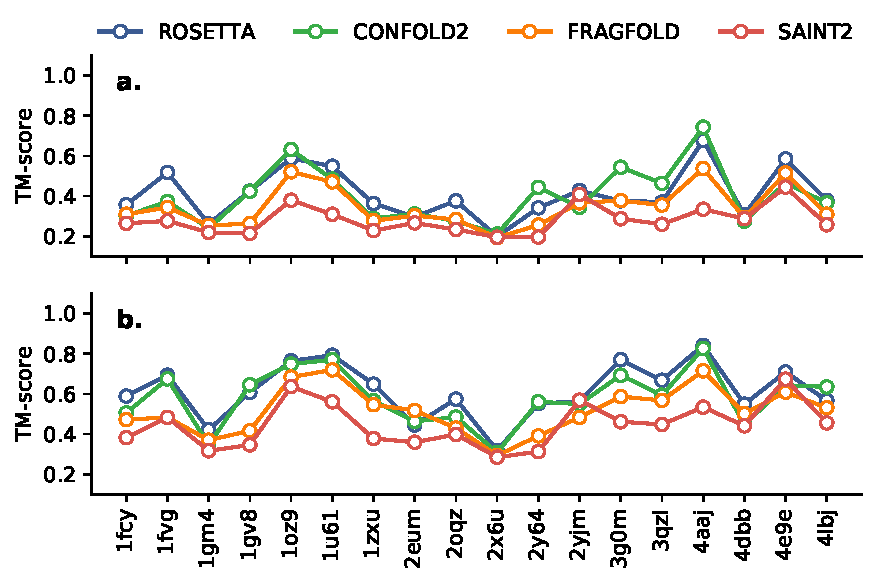
\includegraphics[width=\textwidth]{ample_saint2_tmscoredataincl.pdf}
    \caption[Per-target TM-score analysis for four modelling algorithms with contacts]{Per-target \gls{tmscore} analysis for targets modelled with contact information and four separate \textit{ab initio} structure prediction algorithms. Analysis is subdivided by (a) median \gls{tmscore} of all decoys in each set and (b) \gls{tmscore} of the top-1 decoy in each set.}
    \label{fig:ample_saint2_tmscoredataincl}
\end{figure}

\textcite{Abriata2018-lu} recently attributed the success in the CASP12 experiments to improved accuracy of coevolution-based contact predictors and the availability of many more sequence homologs than ever before. Thus, it is of great interest to explore the structure prediction algorithms in this study with regards to their dependence on the availability of sequence homologs and precise contact predictions.

The results obtained in this study further support the conclusions made by \textcite{Abriata2018-lu} but only for the ROSETTA algorithm. A Spearman's rank-order \gls{cc} analysis of alignment depth and median \gls{tmscore} shows a significant positive correlation for ROSETTA-generated decoy sets (Spearman's $\rho=0.68$, $p<0.01$). This positive correlation is also found for ROSETTA-generated decoy sets with regards to their top-$L$ precision and median \gls{tmscore} (Spearman's $\rho=0.61$, $p<0.01$). All other modelling algorithms do not show a significant correlation, although better decoy sets are generally obtained with greater alignment depths and more precise top-$L$ contacts (\cref{fig:ample_saint2_neffprectm}). Furthermore, the sample size for each correlation analysis was small ($n=18$), and thus further test cases are required for a more confident inference.

\begin{figure}[H]
    \centering
    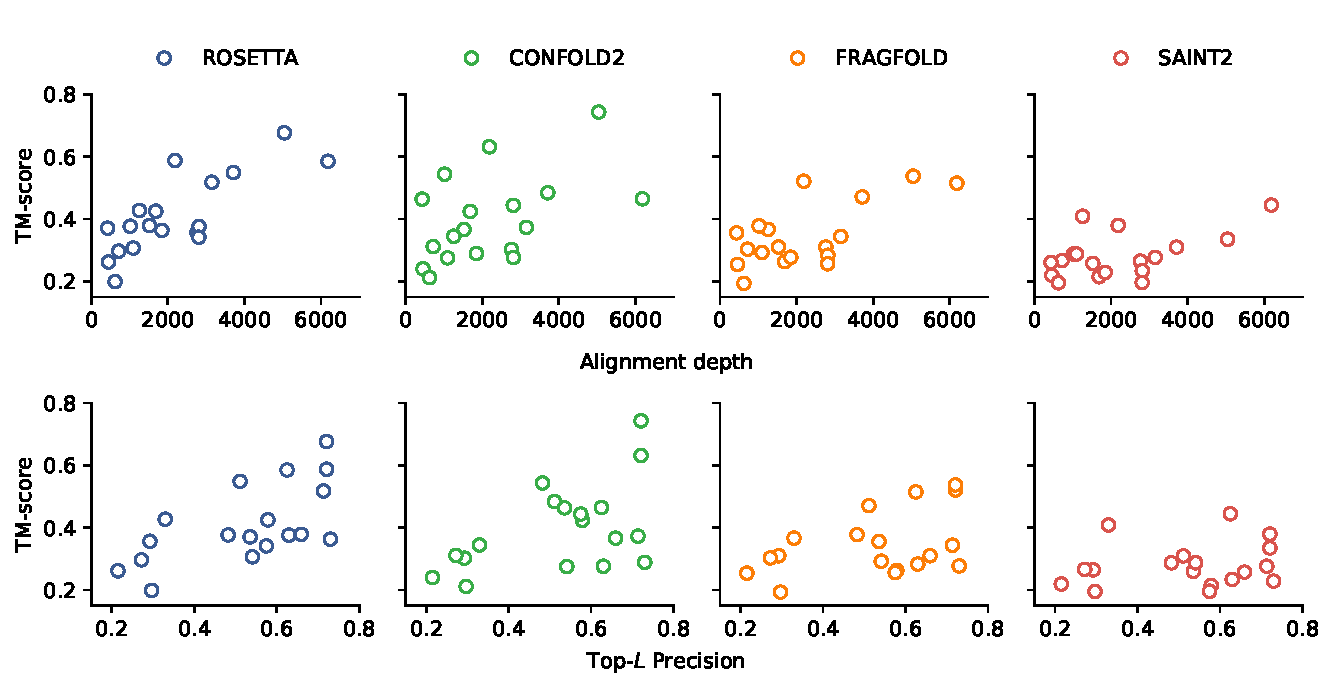
\includegraphics[width=\textwidth]{ample_saint2_neffprectm.pdf}
    \caption[Analysis of alignment depth, precision and TM-scores]{Analysis of median \gls{tmscore} of the contact-based decoy sets and their dependence on  alignment depth and top-$L$ precision.}
    \label{fig:ample_saint2_neffprectm}
\end{figure}

Beyond the use of contact information, parts of this study explored the performance of ROSETTA, FRAGFOLD and SAINT2 when no contact information is provided as distance restraints in \textit{ab initio} structure prediction (CONFOLD2 requires contact information, and thus was excluded). ROSETTA performs best for seven of the nine contact-free decoy sets based on median \gls{tmscore} of the entire decoy set and the \gls{tmscore} of the top-1 decoy (\cref{fig:ample_saint2_tmscoredataexcl}). However, the difference is marginal for the majority of cases. The median values for eight ROSETTA and FRAGFOLD decoy sets differ by less than 0.10 \gls{tmscore} units (seven ROSETTA and SAINT2 sets by less than 0.10 units). Furthermore, the top-1 decoys for only three targets differ greatly between the modelling algorithms, whilst the rest is near identical (\cref{fig:ample_saint2_tmscoredataexcl}).

The top decoy predicted by ROSETTA and SAINT2 based on the sequence of the FAT domain of focal adhesion kinase (\gls{pdb} ID: 1k40) differs by 0.35 \gls{tmscore} units. More significantly though, the top decoy predicted by ROSETTA for the outer surface protein A (\gls{pdb} ID: 2ol8) is considered native-like (\gls{tmscore} $=0.59$), whilst the FRAGFOLD (\gls{tmscore} $=0.35$) and SAINT2 (\gls{tmscore} $=0.24$) counterparts predict incorrect folds. A near-identical scenario applies to the top decoys of the Hypothetical protein PF0907 (\gls{pdb} ID: 4pgo) (ROSETTA \gls{tmscore} $=0.68$; FRAGFOLD \gls{tmscore} $=0.27$; SAINT2 \gls{tmscore} $=0.39$).

\begin{figure}[H]
    \centering
    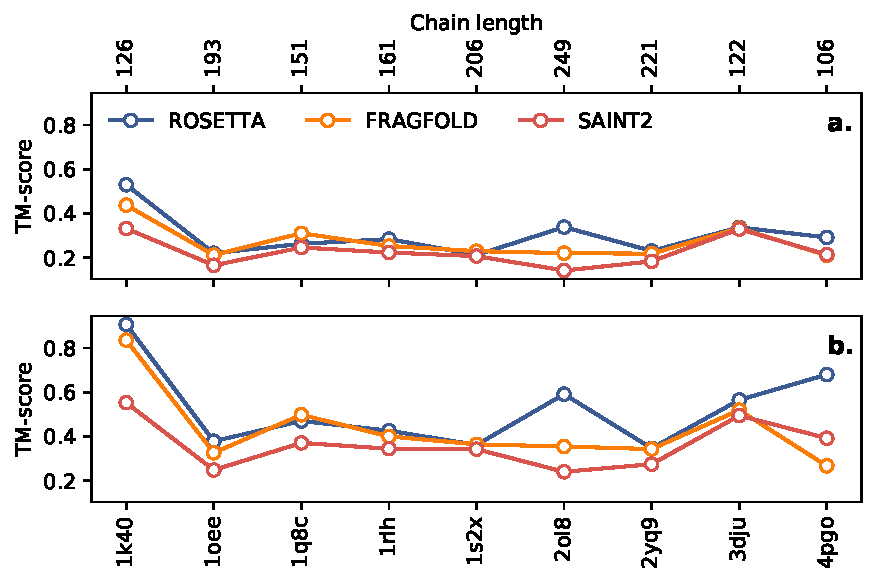
\includegraphics[width=\textwidth]{ample_saint2_tmscoredataexcl.pdf}
    \caption[Per-target TM-score analysis for four modelling algorithms without contacts]{Per-target \gls{tmscore} analysis for targets modelled without contact information and four separate \textit{ab initio} structure prediction algorithms. Analysis is subdivided by (a) median \gls{tmscore} of all decoys in each set and (b) \gls{tmscore} of the top-1 decoy in each set.}
    \label{fig:ample_saint2_tmscoredataexcl}
\end{figure}

An analysis of the modelling results by target fold shows that all-\textalpha\ and mixed \textalpha-\textbeta\ target folds are less challenging to predict than all-\textbeta\ targets (\cref{fig:ample_saint2_tmfoldsize}). The multimodal distributions of all-\textalpha\ and mixed \textalpha-\textbeta\ target decoys predicted by ROSETTA spans from 0.10 \gls{tmscore} units to 0.80. In comparison, the approximately normal distribution for all-\textbeta\ targets by the same algorithm centres at 0.32 \gls{tmscore} units (s.d.=0.08 \gls{tmscore} units). Similarly, FRAGFOLD decoys show a more spread distribution of decoys for all-\textalpha\ and mixed \textalpha-\textbeta\ decoys compared to all-\textbeta. The \gls{tmscore} distributions for CONFOLD2 mixed \textalpha-\textbeta\ and all-\textbeta\ decoys follow multimodal distributions. Whilst this might indicate that CONFOLD2 either predicts the overall target fold correctly or incorrectly, the data might be misleading due to missing targets in the dataset in comparison to the other three modelling algorithms. Lastly, the distributions of \gls{tmscore} for either fold class of SAINT2 decoys appear more similar than the others indicating less difference between the fold classes. However, similarly to the ROSETTA decoys the all-\textbeta\ distribution appears normal whilst the other two are right-skewed highlighting some more accurate decoys in the overall set.

A further subdivision of all target decoys is by target chain length. At the stage of target selection, three main bins were defined from which targets were randomly sampled (see \cref{sec:methods_dataset_predictors}). These bins were defined with target chain length edges of 150 and 200 creating three bins: $0 < x < 150$ \& $150 \leq x < 200$ \& $x \geq 200$ ($x$ refers to the target chain length). A grouping of the decoy \gls{tmscore} by algorithm and target chain length indicates little difference in modelling difficulty (\cref{fig:ample_saint2_tmfoldsize}). Each of the modelling algorithms shows the largest spread for targets with chain lengths in the bin $150 \leq x < 200$. Surprisingly, only FRAGFOLD and SAINT2 performed better for targets in the smallest bin size whilst CONFOLD2 found those targets most challenging. CONFOLD2 also generated the best decoys for one of the largest targets in the dataset (n\textsubscript{res}=216). The set of CONFOLD2 decoys for N-(5-phosphoribosyl)anthranilate isomerase (\gls{pdb} ID: 4aaj) have a median \gls{tmscore} of 0.74 units. ROSETTA decoys show a comparable median \gls{tmscore} of 0.68; however, FRAGFOLD (median \gls{tmscore}=0.54) and SAINT2 (median \gls{tmscore}=0.33) were unable to generate decoys of similarly high quality.

\begin{figure}[H]
    \centering
    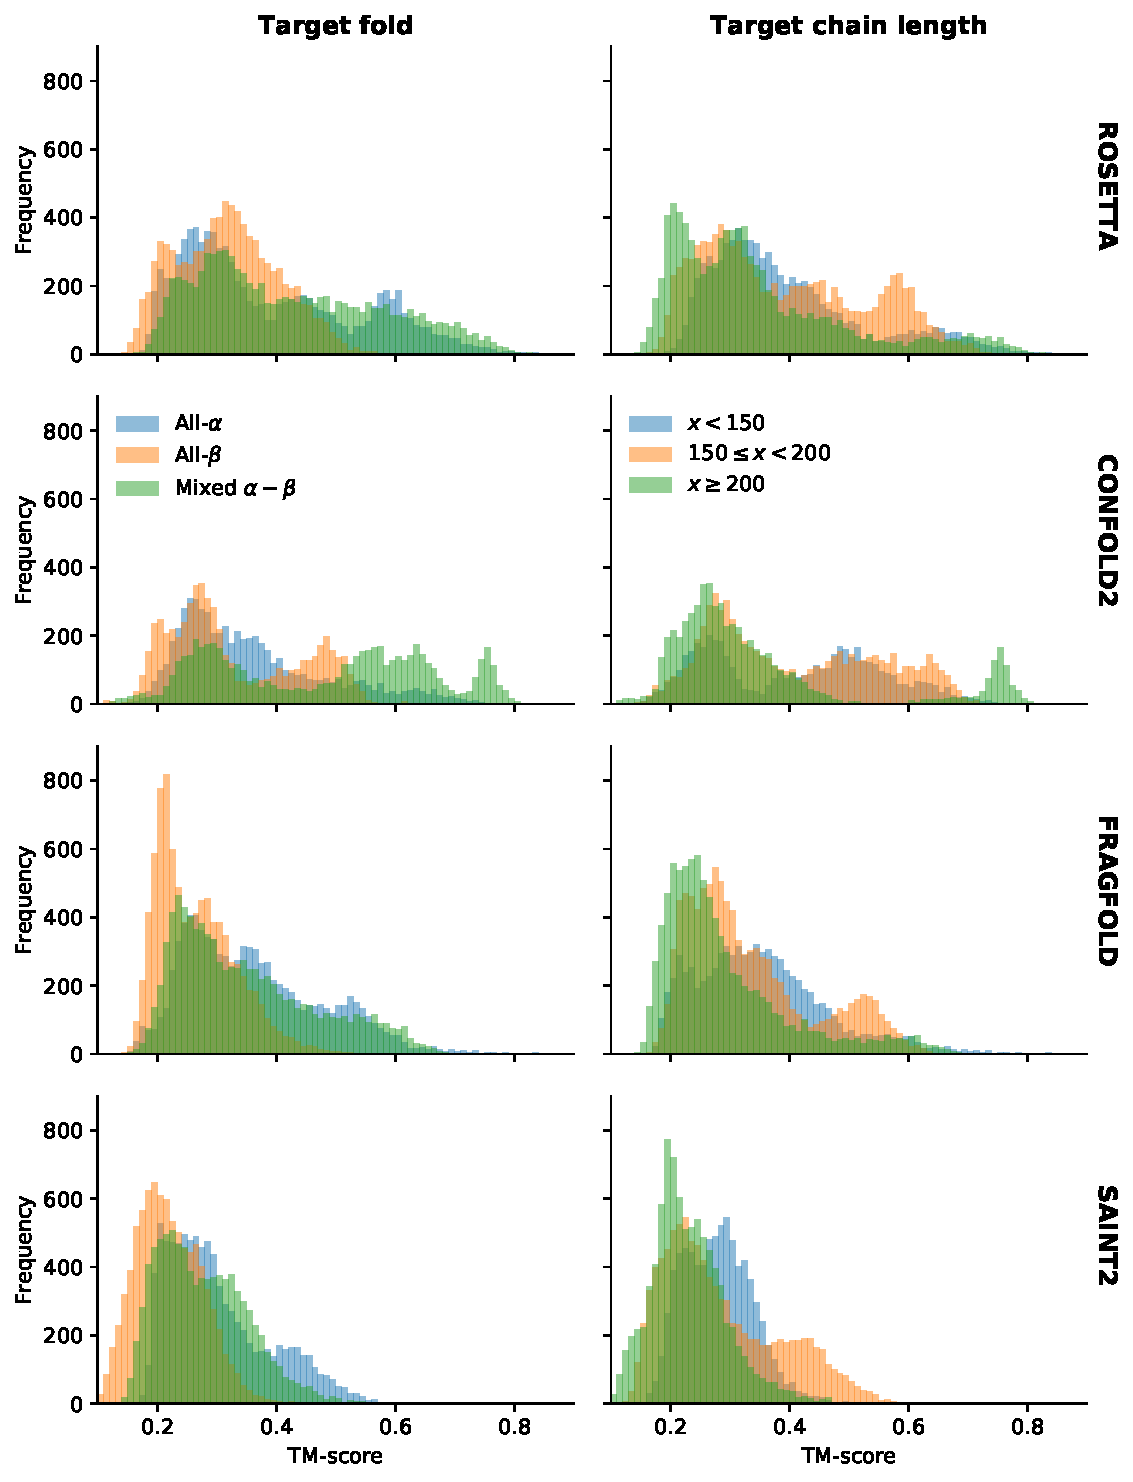
\includegraphics[width=\textwidth]{ample_saint2_tmfoldsize.pdf}
    \caption{Distribution of decoy TM-scores by fold, chain length and algorithm.}
    \label{fig:ample_saint2_tmfoldsize}
\end{figure}

\subsection{Molecular Replacement}
The final step in this study was to explore the benefits or drawbacks of each \textit{ab initio} structure prediction algorithm for \gls{mr}.

Each \textit{ab initio} modelling-algorithm generated at least two decoy sets sufficient for \gls{mr} structure solution (\cref{fig:ample_saint2_mrsuccess}). ROSETTA and SAINT2 decoy sets led to the solutions of five targets each, whilst FRAGFOLD decoys solved four and CONFOLD2 decoys just two. All four algorithms predicted decoys of good enough quality to solve the structures of the Hypothetical protein AQ\_1354 (\gls{pdb} ID: 1oz9) and Putative Ribonuclease III (\gls{pdb} ID: 1u61), although SAINT2-based AMPLE search models yielded the highest ratio of successful search models compared to the total trialled in both cases (\cref{fig:ample_saint2_mrsuccess}). Besides these two targets, little consensus exists amongst the targets for which structure solutions were obtained across the different modelling algorithms.

\begin{figure}[H]
    \centering
    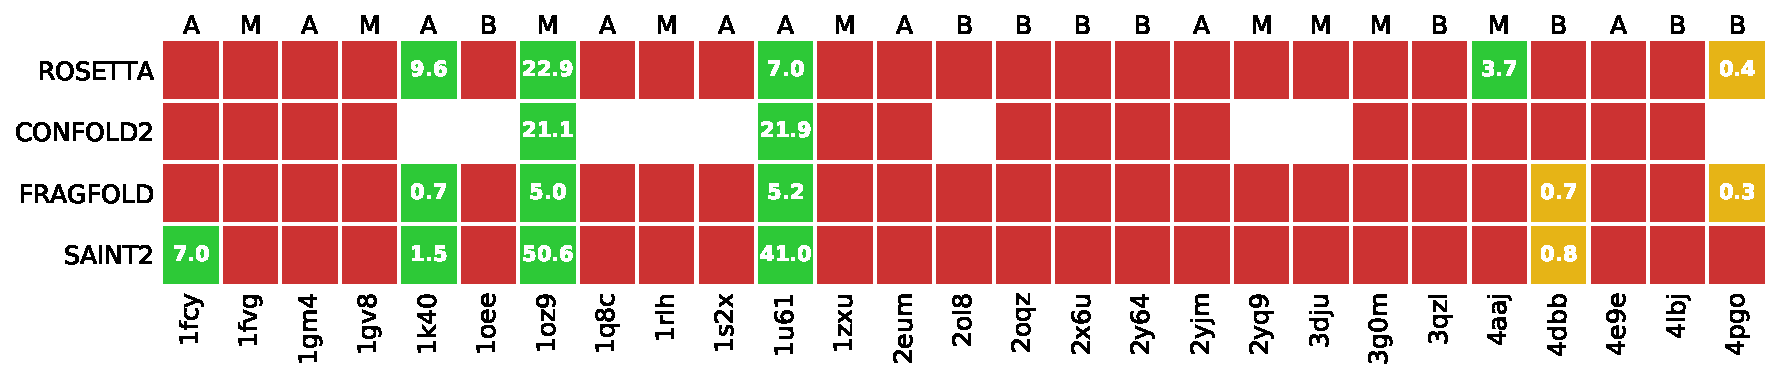
\includegraphics[width=\textwidth]{ample_saint2_mrsuccess.pdf}
    \caption[Summary of MR success with AMPLE ensemble search models.]{Summary of MR success with AMPLE ensemble search models. Search models are based on decoy sets generated with different \textit{ab initio} structure prediction protocols. The colour coding indicates structure solution: no solution (red), one solution (orange), more than one solution (green). The number in cells with at least one solution states the percentage of successful search models. The one-letter codes above each column indicate the target fold: all-\textalpha\ (A); all-\textbeta\ (B); mixed \textalpha-\textbeta\ (M). The row labelled ``IDEALH'' refers to AMPLE's ideal helix run.}
    \label{fig:ample_saint2_mrsuccess}
\end{figure}

The chain length for targets with structure solutions ranges from 106 (\gls{pdb} ID: 4pgo) to 236 (\gls{pdb} ID: 1fcy) residues. Although statistics cannot reliable indicate the performance with such a small sample size, SAINT2 decoys solve on average the largest targets (mean target chain length ROSETTA=147, CONFOLD2=144, FRAGFOLD=136,  SAINT2=162). The ROSETTA, FRAGFOLD and SAINT2 decoys achieved structure solutions for all three fold classifications, whilst CONFOLD2 did not solve for any all-\textbeta\ target. Nevertheless, successful AMPLE ensemble search models for all-\textbeta\ targets derived from the former three algorithms were scarce with only a single one leading to structure solution (\cref{fig:ample_saint2_mrsuccess}).

The difference in overall decoy quality between the four different \textit{ab initio} structure prediction algorithms is further noticed in the successful AMPLE-generated ensemble search models. ROSETTA decoys result in more complete AMPLE ensemble search models, which lead to structure solution (\cref{fig:ample_saint2_tlevelssdist}). Although CONFOLD2 has a similar maximum of just under 100\% completeness, 75\% of all successful search models contained at most 40\% of the target sequence. Overall, FRAGFOLD decoys translated into the least complete successful AMPLE search models with 75\% containing less than 20\% of the target sequence. SAINT2 has the shortest range spanning from 8\% to 70\% target completeness.

\begin{figure}[H]
    \centering
    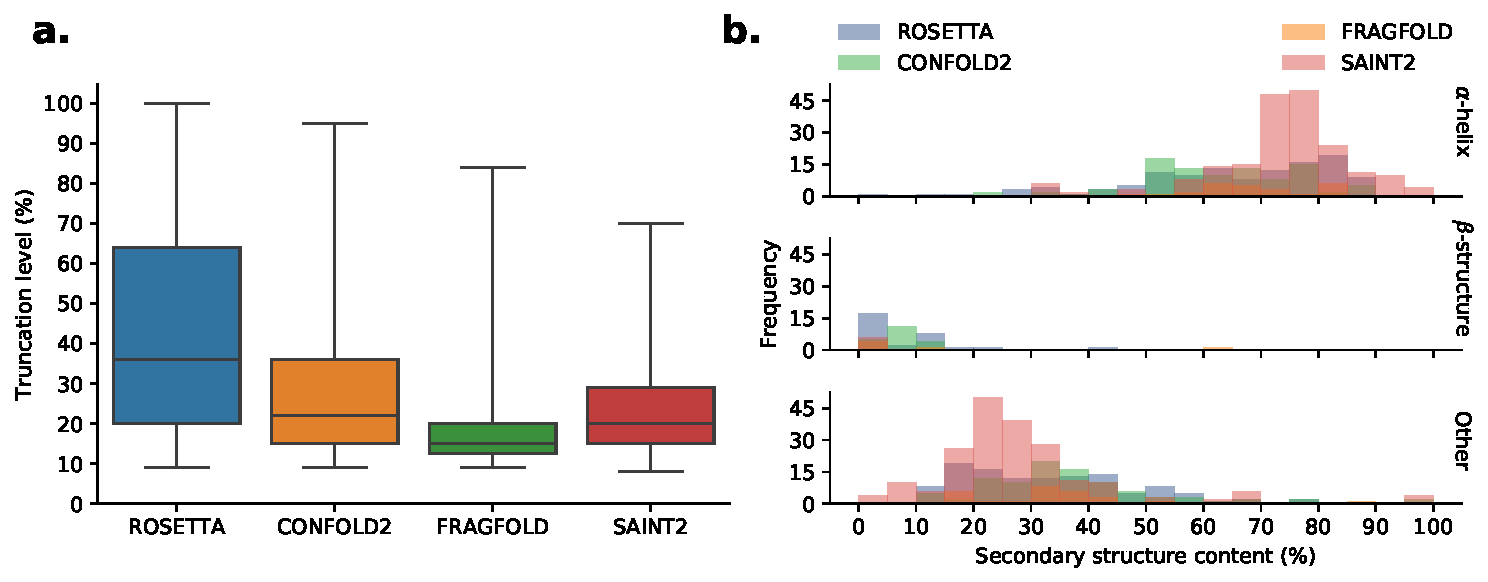
\includegraphics[width=\textwidth]{ample_saint2_tlevelssdist.pdf}
    \caption[Distribution of search model truncation and secondary structure content]{Distribution of (a) search model truncation and (b) secondary structure content for successful AMPLE ensemble search models given decoys from four \textit{ab initio} structure prediction algorithms. Secondary structure for each ensemble search model evaluated with DSSP \cite{Frishman1995-si}.}
    \label{fig:ample_saint2_tlevelssdist}
\end{figure}

An inspection of the secondary structure content of all successful ensemble search models outlines an important difference between SAINT2 and the other three modelling algorithms. Successful search models derived from SAINT2 decoys are predominantly \textalpha-helical (\cref{fig:ample_saint2_tlevelssdist}). An analysis of the secondary structure makeup, as assigned by DSSP \cite{Frishman1995-si}, shows that successful SAINT2 search models contain approximately 70-80\% \textalpha-helices with the rest being unassigned secondary structure. In comparison, the successful ensemble search models from other modelling algorithms contain a range from 50-90\% \textalpha-helices, whilst the remainder is either unstructured or \textbeta-structure (\cref{fig:ample_saint2_tlevelssdist}).

This important observation is crucial in assessing the structure solutions obtained since simple helices could be derived from idealised \textalpha-helix libraries and save the great overhead of predicting, preparing and sampling decoys in AMPLE. A visual inspection of SAINT2 ensemble search models highlights that the FAT domain of focal adhesion kinase (\gls{pdb} ID: 1k40) and the Amyloid-\textbeta\ A4 precursor protein-binding family A1(\gls{pdb} ID: 4dbb) were solved with single \textalpha-helices (\cref{fig:ample_saint2_betaex}). Trialling the experimental data of these targets against AMPLE's ideal helix library \cite{Thomas2015-wu} shows that the former could have been solved without the modelling overhead. In fact, SAINT2 decoys did not result in any additional structure solutions compared to AMPLE's ideal helix library except for the solution of the A4 precursor protein-binding family A1(\gls{pdb} ID: 4dbb) (\cref{fig:ample_saint2_mrsuccess}). In comparison, the other modelling algorithms resulted in similar idealised fragments, especially in borderline cases (\cref{fig:ample_saint2_betaex}). However, these fragments are not strictly \textalpha-helical, and thus would require more sophisticated and computationally complex idealised-fragment library generation protocols \cite[e.g.,][]{Jenkins2018-gf} or libraries of recurring tertiary structure motifs \cite[e.g.,][]{Sammito2013-ug}. Nevertheless, even the most sensitive \gls{mr} ideal-fragment-selection algorithms could almost certainly not identify a search model of similar quality to that derived from ROSETTA decoys for the Hypothetical protein PF0907 (\gls{pdb} ID: 4pgo)(\cref{fig:ample_saint2_betaex}), which might be essential in structure solution determination of some targets.

\begin{figure}[H]
    \centering
    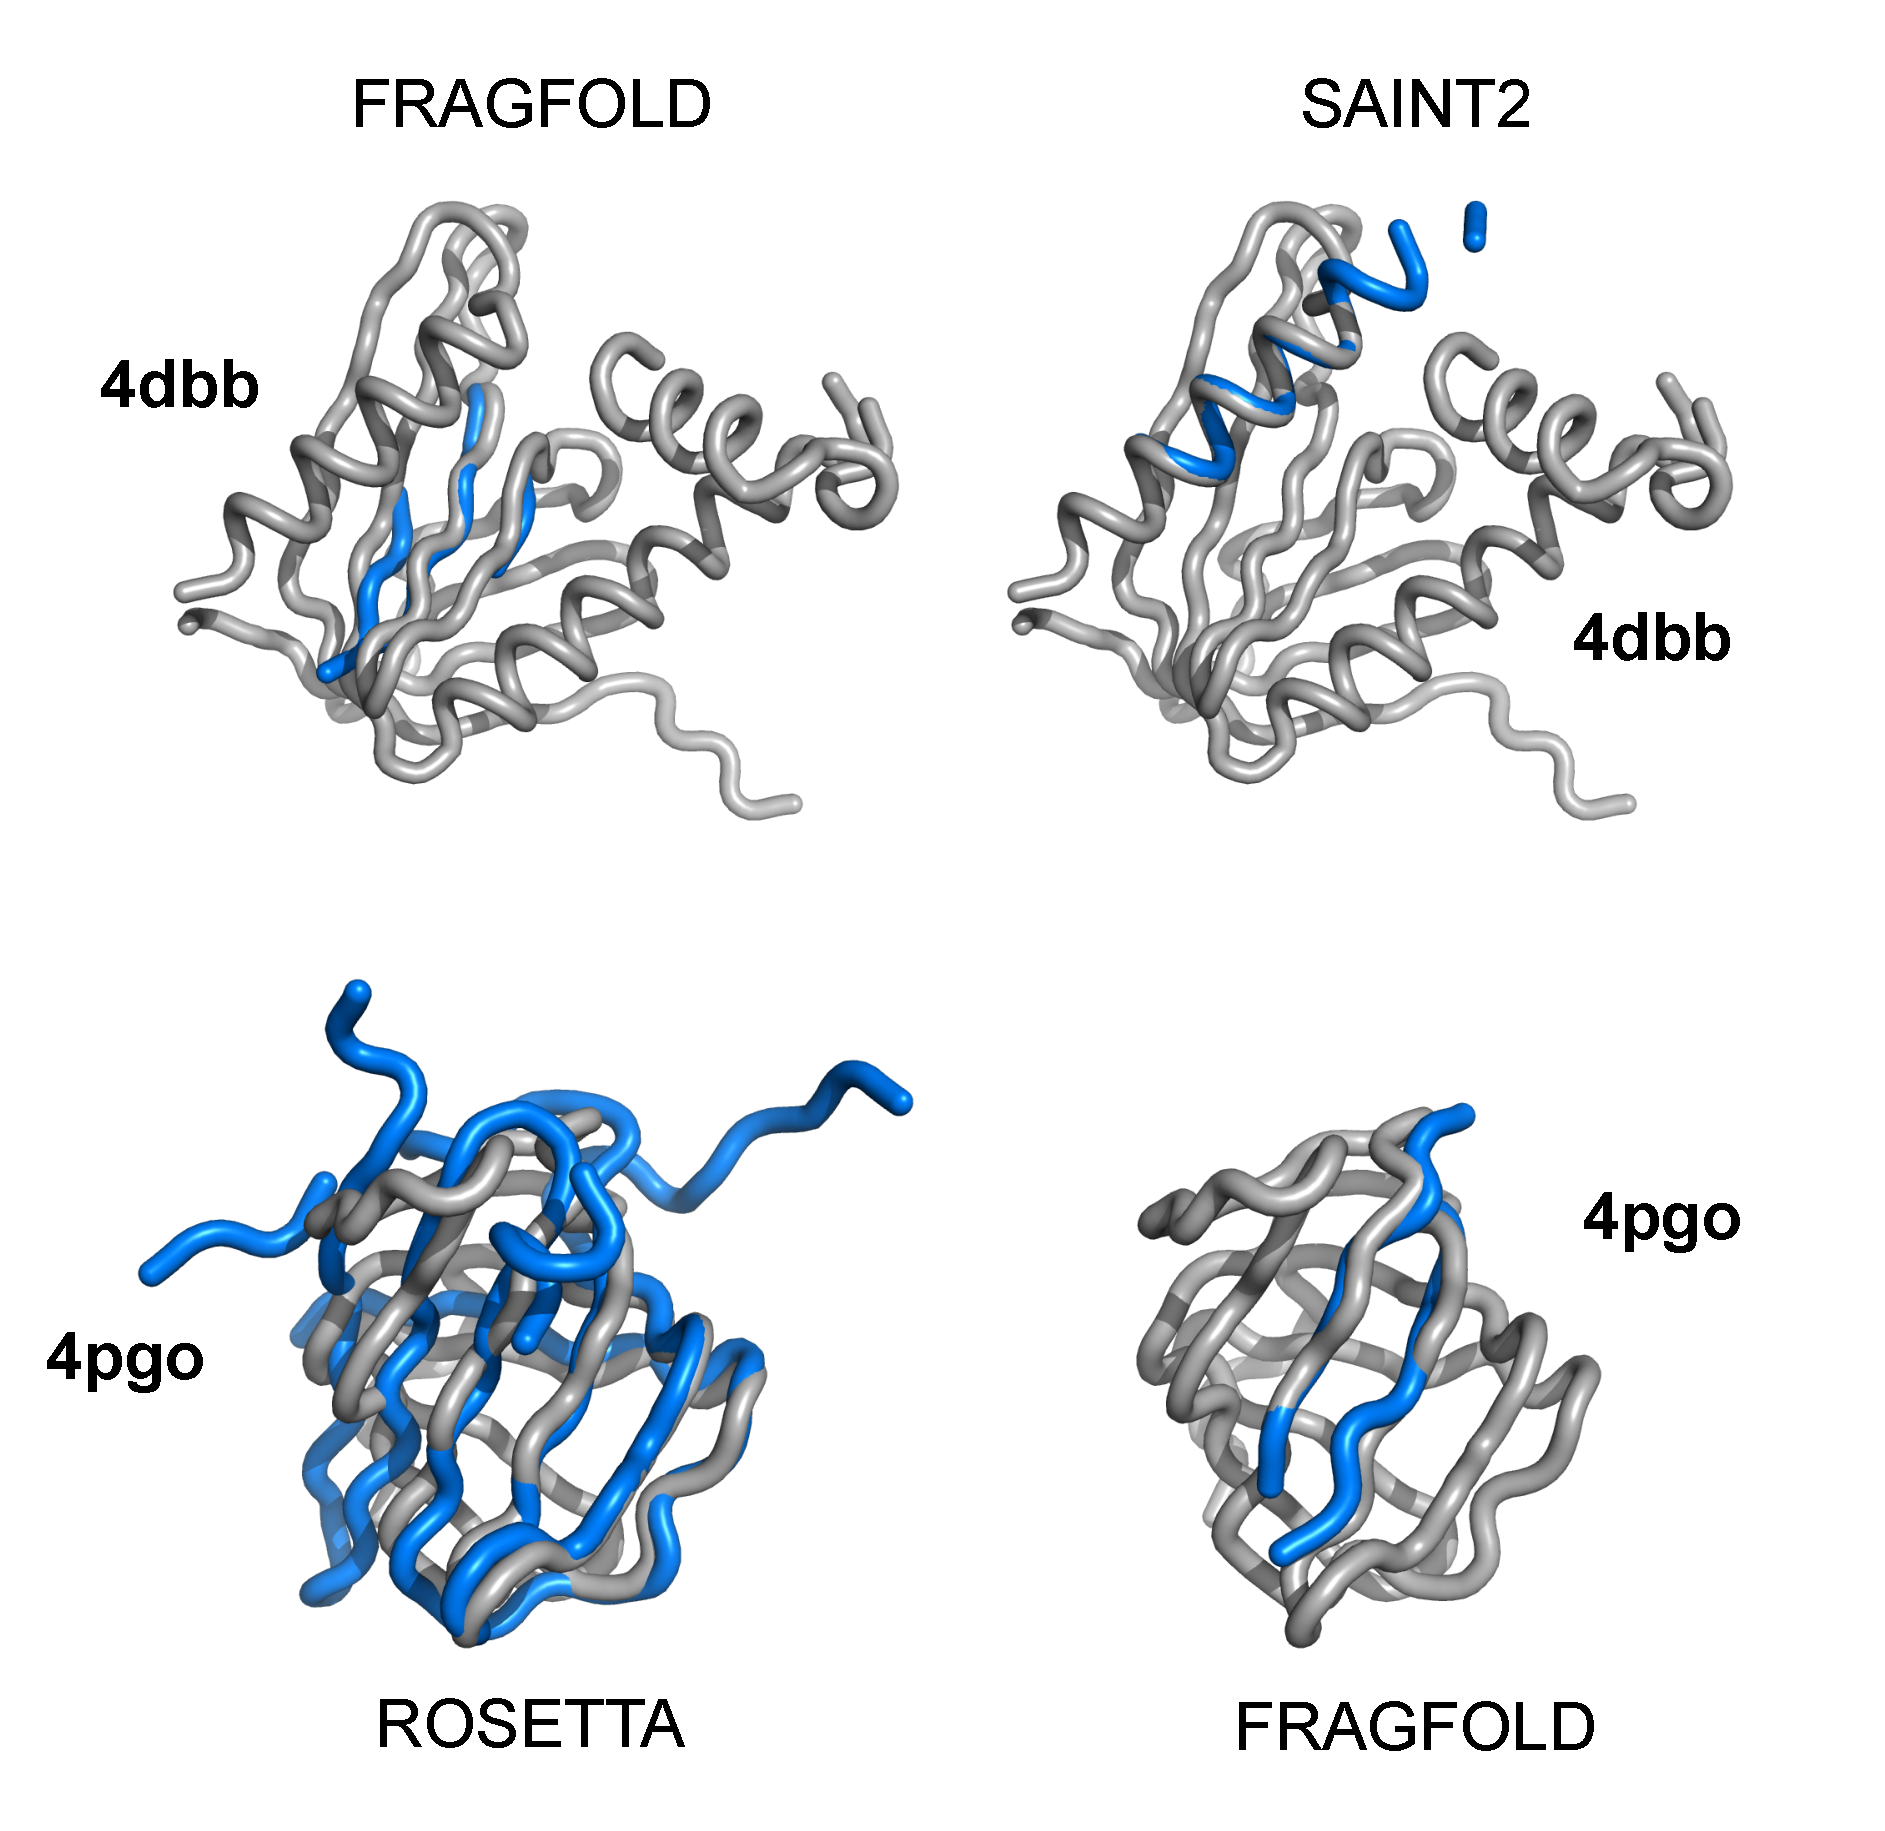
\includegraphics[width=\textwidth]{ample_saint2_betaex.pdf}
    \caption[Examples of PHASER-placed AMPLE search models.]{Examples of PHASER-placed AMPLE search models that led to structure solution. AMPLE search models are coloured blue and deposited structures in gray. The \gls{pdb} identifiers and modelling protocol given alongside each example.}
    \label{fig:ample_saint2_betaex}
\end{figure}

Whilst all \textit{ab initio} structure prediction algorithms enabled structure solutions of at least two targets, the relationship between the quality of the starting decoys and \gls{mr} structure solution success needs to be evaluated. ROSETTA and CONFOLD2 generated the highest quality decoys, followed by FRAGFOLD and SAINT2 (\cref{fig:ample_saint2_tmscoredist}). Thus, most structure solutions would have been expected for the former two since more native-like decoys are generally better search models. However, an analysis of the \gls{rmsd} of each ensemble search model's centroid shows that decoy quality may not always be the most reliable indicator. Although search models are often considered suitable once their \gls{rmsd} to the native structure is better than 1.5\AA \cite{Scapin2013-yp}, this threshold does not strictly apply to \textit{ab initio} modelling-based AMPLE ensemble search models (\cref{fig:ample_saint2_mrstats}). For example, a small number of SAINT2-derived search models, which were prepared for the FAT domain of focal adhesion kinase (\gls{pdb} ID: 1k40), exceed this threshold greatly with \gls{rmsd} values $>10$\AA\ (up to 28\AA) yet resulting in PHASER \gls{llg} values in excess of the success threshold of 60 \cite{Oeffner2018-ur}. Additionally, nearly 25\% of all successful ensemble search models have \gls{rmsd} values $\geq2$\AA\ and PHASER \gls{llg} scores of $\geq$60. Although striking at first, structure solutions in these situations are often achieved by out-of-sequence-register placement of search models. An analysis of the \gls{rio} score metric shows that the usefully placed parts of all but one AMPLE search model with \gls{rmsd} value greater than 10\AA\ is out-of-register. Furthermore, it is important to remember that \gls{rmsd} values greatly differ based on the optimal superposition of the model and target.

\begin{figure}[H]
    \centering
    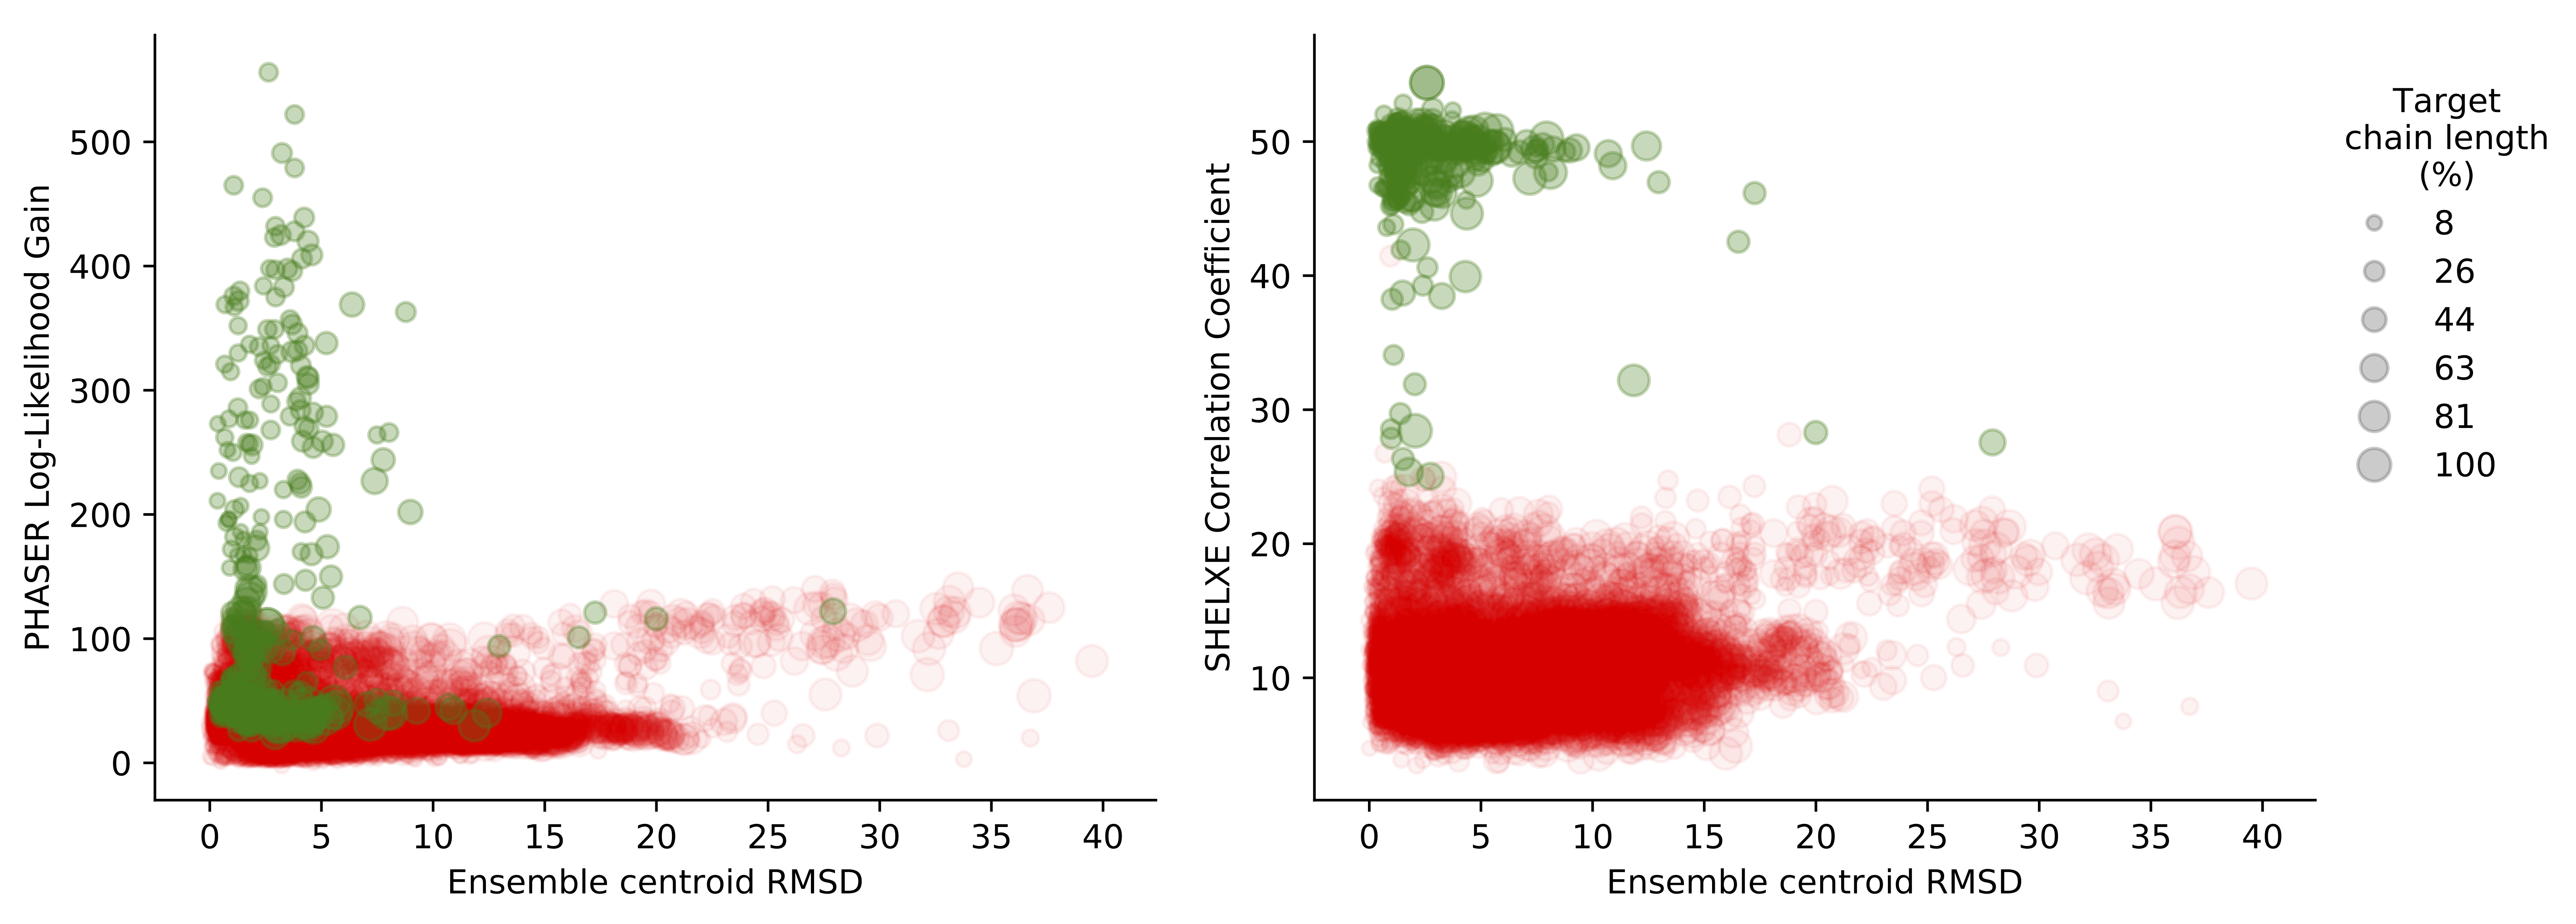
\includegraphics[width=\textwidth]{ample_saint2_mrstats.pdf}
    \caption[Relationship between ensemble quality, PHASER LLG and SHELXE CC]{Relationship between ensemble quality, PHASER \gls{llg} and SHELXE \gls{cc}. Data points are coloured based on the outcome of their \gls{mr} trials: green indicate structure solution, red indicate no structure solution.}
    \label{fig:ample_saint2_mrstats}
\end{figure}

Lastly, one characteristic of a good \gls{mr} search model is good stereochemical geometry of its peptide-chain backbone, especially during refinement. Fragment-based structure prediction algorithms typically contain good stereochemistry, because the template fragments are derived from refined protein structures. In comparison, CONFOLD2, which does not use fragments, relies on physics-based energy functions to identify good stereochemistry of the decoy backbone. Thus, it is important to understand if poor stereochemistry is present CONFOLD2 ensemble search models, such that it might explain why good decoy quality does not translate to more \gls{mr} structure solutions.

Indeed, a Ramachandran analysis of \textphi\ and \textpsi\ peptide backbone angles outlines much poorer stereochemistry of ensemble search model centroids for CONFOLD2 compared to all fragment-assembly-based structure prediction algorithms (\cref{fig:ample_saint2_ramach}). ROSETTA search models, which are made up of crudely-refined decoys, possess at most 2\% of residues as outliers. SAINT2, which might not outcompete other protocols in overall quality, shows the second best stereochemistry of centroid models without any refinement.  FRAGFOLD contains around 5\% outliers for the majority of search models. In comparison to these statistics CONFOLD2 contains around 5-15\% Ramachandran outliers in centroid decoys. 

\begin{figure}[H]
    \centering
    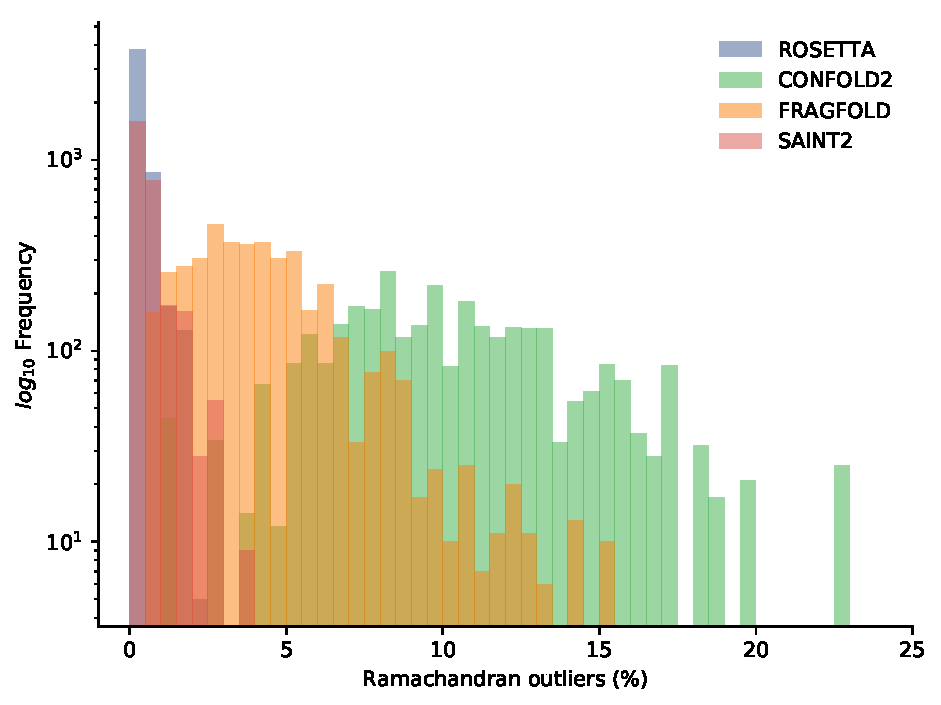
\includegraphics[width=0.7\textwidth]{ample_saint2_ramach.pdf}
    \caption[Distribution of Ramachandran outliers of AMPLE ensemble search model centroids]{Distribution of Ramachandran outliers of AMPLE ensemble search model centroids based on decoys predicted with four \textit{ab initio} structure prediction protocols. Outliers were calculated using PyRAMA (\href{https://github.com/gerdos/PyRAMA}{https://github.com/gerdos/PyRAMA}).}
    \label{fig:ample_saint2_ramach}
\end{figure}

Further analysis of the centroids of each truncated AMPLE ensemble demonstrates the importance of good stereochemistry for success. Out of 94 successful ensemble search models only 17 contain outliers. This contrasts to over 390 unsuccessful ensemble search models with TM-scores greater than 0.5 units and on average 6\% outliers (min\textsubscript{outliers}=1\%; max\textsubscript{outliers}=23\%). However, perfect peptide backbone stereochemistry is still no guarantee for \gls{mr} structure solution. The centroids of over 200 unsuccessful CONFOLD2 ensemble search models have TM-scores of at least 0.5 units with residue counts ranging from 6 to 106.

\section{Discussion}
In this chapter, work was conducted to explore \textit{ab initio} protein structure prediction protocols as alternatives to ROSETTA and QUARK. Three algorithms --- CONFOLD2, FRAGFOLD and SAINT2 --- were trialled on a set of 27 globular targets to evaluate their performance with regards to structure prediction and subsequent \gls{mr} trials.

The experiments in this study highlighted that ROSETTA remains the most accurate structure prediction protocol amongst the trialled ones. ROSETTA outperformed the other three algorithms across the majority of protein targets for entire decoy sets and the best decoy in each set. These findings were further confirmed in the latest CASP12 experiments, which outlined ROSETTA's success compared to other protocols \cite{Ovchinnikov2017-wp,Abriata2018-lu}. Furthermore, the findings describing the comparable performance of ROSETTA and CONFOLD2 \cite{Adhikari2018-lj,Michel2017-xh} are supported in this work. Given that the latter relies entirely on the provided contact information, such performance emphasises the quality and importance of contact prediction in protein structure modelling. It is also to be expected that the increase in sequence availability will improve the decoy quality further \cite{Abriata2018-lu,Schaarschmidt2018-mh}.

In this study, the alternative fragment-assembly based algorithms FRAGFOLD and SAINT2 were tested. Although both did predict native-like decoys for some targets, their performance was overall much worse than ROSETTA and CONFOLD2. In particular, SAINT2 did not generate decoys of native-like quality in cases where all other algorithms did. Beyond overall decoy quality, previous findings suggested a difference in difficulty based on the target fold. These findings are further manifested here. All algorithms predicted most native-like decoys for all-\textalpha\ and mixed \textalpha-\textbeta\ targets. Although previous studies also reported on greater difficulty for larger targets --- especially in cases without contact information --- such findings could not be confirmed here.

Given that the application of these decoys is primarily aimed at challenging targets in \gls{mr}, the quality of decoys is not necessarily enough to predict the success of AMPLE-generated search models. The results in this chapter clearly that CONFOLD2 generates high quality decoys, which do not translate into \gls{mr} search models suitable for routine structure solution. Despite a recent example of the successful application of \gls{cns}-generated decoys in \gls{mr} \cite{Sjodt2018-zq}, further research is required to identify the main bottleneck observed in this study. ROSETTA, FRAGFOLD and SAINT2 achieved structure solutions for a number of targets, despite poor decoy quality in cases of the latter two. CONFOLD2 decoys appear to suffer from poor stereochemistry, and results suggest that decoy refinement might be essential to exploit the underlying decoy quality.

In conclusion, ROSETTA remains the best modelling algorithm for unconventional \gls{mr} in AMPLE. Although some of this success must be due to the fact that AMPLE's algorithm is tailored towards exploiting the cluster variance derived from ROSETTA decoys, it cannot be downplayed that ROSETTA generates the most accurate decoys overall. However, it is crucial to investigate whether CONFOLD2 decoys, potentially remodelled to improve the backbone stereochemistry, might provide a suitable routine alternative to ROSETTA, especially because fragment databases are not required and modelling time per decoy is reduced by approximately a factor of four.
